\documentclass[codesnippet]{jss}
%\documentclass[nojss]{jss}

%% -- LaTeX packages and custom commands ---------------------------------------

%% recommended packages
\usepackage{thumbpdf,lmodern}
\usepackage{amssymb}
\usepackage{amsmath}

%% another package (only for this demo article)
\usepackage{framed}

%% new custom commands
\newcommand{\class}[1]{`\code{#1}'}
\newcommand{\fct}[1]{\code{#1()}}

\newcommand{\RBnote}[1]{\textcolor{red}{#1}}

%\hyphenation{Fa-sa-no=Fran-ces-chi-ni}

%% -- Article metainformation (author, title, ...) -----------------------------

%% - \author{} with primary affiliation
%% - \Plainauthor{} without affiliations
%% - Separate authors by \And or \AND (in \author) or by comma (in \Plainauthor).
%% - \AND starts a new line, \And does not.
\author{Elan Ness-Cohn\\Northwestern University
   \And Rosemary Braun\\Northwestern University}
\Plainauthor{Elan Ness-Cohn, Rosemary Braun}

%% - \title{} in title case
%% - \Plaintitle{} without LaTeX markup (if any)
%% - \Shorttitle{} with LaTeX markup (if any), used as running title
\title{Fasano--Franceschini Test: an Implementation of a 2-Dimensional Kolmogorov--Smirnov test in \proglang{R}}
\Plaintitle{Fasano--Franceschini Test: an Implementation of a 2-Dimensional Kolmogorov--Smirnov test in R}
\Shorttitle{2-dimensional KS test in \proglang{R}}

%% - \Abstract{} almost as usual
\Abstract{
The univariate Kolmogorov-Smirnov (KS) test is a non--parametric
statistical test designed to assess whether a set of data is
consistent with a given probability distribution (or, in the two-sample
case,  whether the two
samples come from the same underlying distribution).
The versatility of the KS test has
made it a cornerstone of statistical analysis and is commonly used
across the scientific disciplines. However, the test proposed by
Kolmogorov and Smirnov does not naturally extend to multidimensional
distributions.  Here, we present the \pkg{fasano.franceschini.test}
package, an  \proglang{R} implementation of the 2-D KS two--sample
test as defined by Fasano and Franceschini~\citep{Fasano1987}. The
\pkg{fasano.franceschini.test} package provides three improvements
over the current 2-D KS test on the Comprehensive \proglang{R} Archive
Network (CRAN): (i) the Fasano and Franceschini test has been shown to
run in $O(n^2)$ versus the Peacock implementation which runs in
$O(n^3)$; (ii) the package implements a procedure for handling ties in
the data; and (iii) the package implements a parallelized
bootstrapping procedure for improved significance testing. Ultimately,
the \pkg{fasano.franceschini.test} package presents a robust
statistical test for analysing random samples defined in 2-dimensions.
}

%% - \Keywords{} with LaTeX markup, at least one required
%% - \Plainkeywords{} without LaTeX markup (if necessary)
%% - Should be comma-separated and in sentence case.
\Keywords{Fasano--Franceschini test, 2-D Kolmogorov--Smirnov test, Multivariate, KS test, \proglang{R}}
\Plainkeywords{Fasan--Franceschini test, 2-D Kolmogorov--Smirnov test, Multivariate, KS test,  R}

%% - \Address{} of at least one author
%% - May contain multiple affiliations for each author
%%   (in extra lines, separated by \emph{and}\\).
%% - May contain multiple authors for the same affiliation
%%   (in the same first line, separated by comma).
\Address{
  Elan Ness-Cohn\\
  Department of Molecular Biosciences\\
  \emph{and}\\
  NSF-Simons Center for Quantitative Biology\\
  Northwestern University\\
  Evanston, IL 60208\\
  E-mail: \email{elan.ness-cohn@northwestern.edu}\\
  URL: \url{https://www.nesscoder.com}\\

Rosemary Braun\\
  Department of Molecular Biosciences,\\
  Department of Engineering Sciences and Applied Mathematics,\\
  Department of Physics and Astronomy,\\
  Northwestern Institute on Complex Systems,\\
  \emph{and}\\
  NSF-Simons Center for Quantitative Biology\\
  Northwestern University\\
  Evanston, IL 60208\\
  E-mail: \email{rbraun@northwestern.edu}\\
  URL: \url{https://sites.northwestern.edu/braunlab/}\\

}
\begin{document}

%% -- Introduction -------------------------------------------------------------

%% - In principle "as usual".
%% - But should typically have some discussion of both _software_ and _methods_.
%% - Use \proglang{}, \pkg{}, and \code{} markup throughout the manuscript.
%% - If such markup is in (sub)section titles, a plain text version has to be
%%   added as well.
%% - All software mentioned should be properly \cite-d.
%% - All abbreviations should be introduced.
%% - Unless the expansions of abbreviations are proper names (like "Journal
%%   of Statistical Software" above) they should be in sentence case (like
%%   "generalized linear models" below).

\section[Introduction]{Introduction} \label{sec:intro}

The Kolmogorov--Smirnov (KS) is a non--parametric, univariate
statistical test designed to assess whether a set of data is
consistent with a given probability distribution (or, in the two-sample
case,  whether the two
samples come from the same underlying distribution). First derived by
Kolmogorov and Smirnov in a series of
papers~\citep{Kolmogorov1933,Kolmogorov1933a,Smirnov1936,Smirnov1937,Smirnov1939,Smirnov1944,Smirnov1948},
the one-sample KS test defines the distribution of the quantity
$D_{KS}$, the maximal absolute difference between the empirical
cumulative distribution function (CDF) of a set of values and a
reference probability distribution. Kolmogorov and Smirnov's key
insight was proving the distribution of $D_{KS}$ was independent of
the CDFs being tested. Thus, the test can effectively be used to
compare any univariate empirical data distribution to any continuous
univariate reference distribution. The two-sample KS test could further
be used to compare any two univariate empirical data distributions
against each other to determine if they are drawn from the same
underlying univariate distribution.

The nonparametric versatility of the univariate KS test has made it a cornerstone of
statistical analysis and is commonly used across the scientific
disciplines~\citep{Atasoy2017,Chiang2018,Hahne2018,Hargreaves2020,Wong2020,Kaczanowska2021}.
However, the KS test as proposed by Kolmogorov
and Smirnov does not naturally extend to distributions in more
than one dimension. Fortunately, a solution to the dimensionality
issue was articulated by Peacock~\citep{Peacock1983} and later
extended by Fasano and Franceschini~\citep{Fasano1987}.

Currently, only the Peacock implementation of the 2-D two-sample KS
test is available in \proglang{R}~\citep{R} with the
\pkg{Peacock.test} package via the \fct{peacock2} function, but this
has been shown to be markedly slower than the Fasano and Franceschini
algorithm~\citep{Lopes2007}. A \proglang{C} implementation of the
Fasano--Franceschini test is available in~\cite{numericalRecipes};
however, arguments have been made to the validity of the
implementation of the test not being
distribution-free~\citep{Babu2006}. Furthermore, in the \proglang{C}
implementation, statistical testing is based on a fit to Monte Carlo
simulation that is only valid for significance levels $\alpha \lessapprox 0.20$.

Here we present the \pkg{fasano.franceschini.test} package as an
\proglang{R} implementation of the 2-D two-sample KS test described
by Fasano and Franceschini~\citep{Fasano1987}. The
\pkg{fasano.franceschini.test} package provides two improvements over
the current 2-D KS test available on the Comprehensive \proglang{R} Archive
Network (CRAN): (i) the Fasano and Franceschini test has been shown to
run in $O(n^2)$ versus the Peacock implementation which runs in
$O(n^3)$; and (ii) the package implements a bootstrapping procedure
for improved significance testing and mitigates the limitations of
the test brought noted by~\citet{Babu2006}.

\section{Models and software} \label{sec:models}

\subsection{1-D Kolmogorov--Smirnov Test}

The Kolmogorov--Smirnov (KS) test is a non--parametric method for
determining whether a sample is consistent with a given probability
distribution~\citep{Stephens1992a}.
%
In one dimension, the Kolmogorov-Smirnov statistic ($D_{KS}$) is the
defined by the maximum absolute difference between the cumulative
density functions of the data and model (one--sample), or between the
two data sets (two--sample), as illustrated in
\textbf{Figure~\ref{fig:kstest1D}}.

\begin{figure}[hbt]
\centering
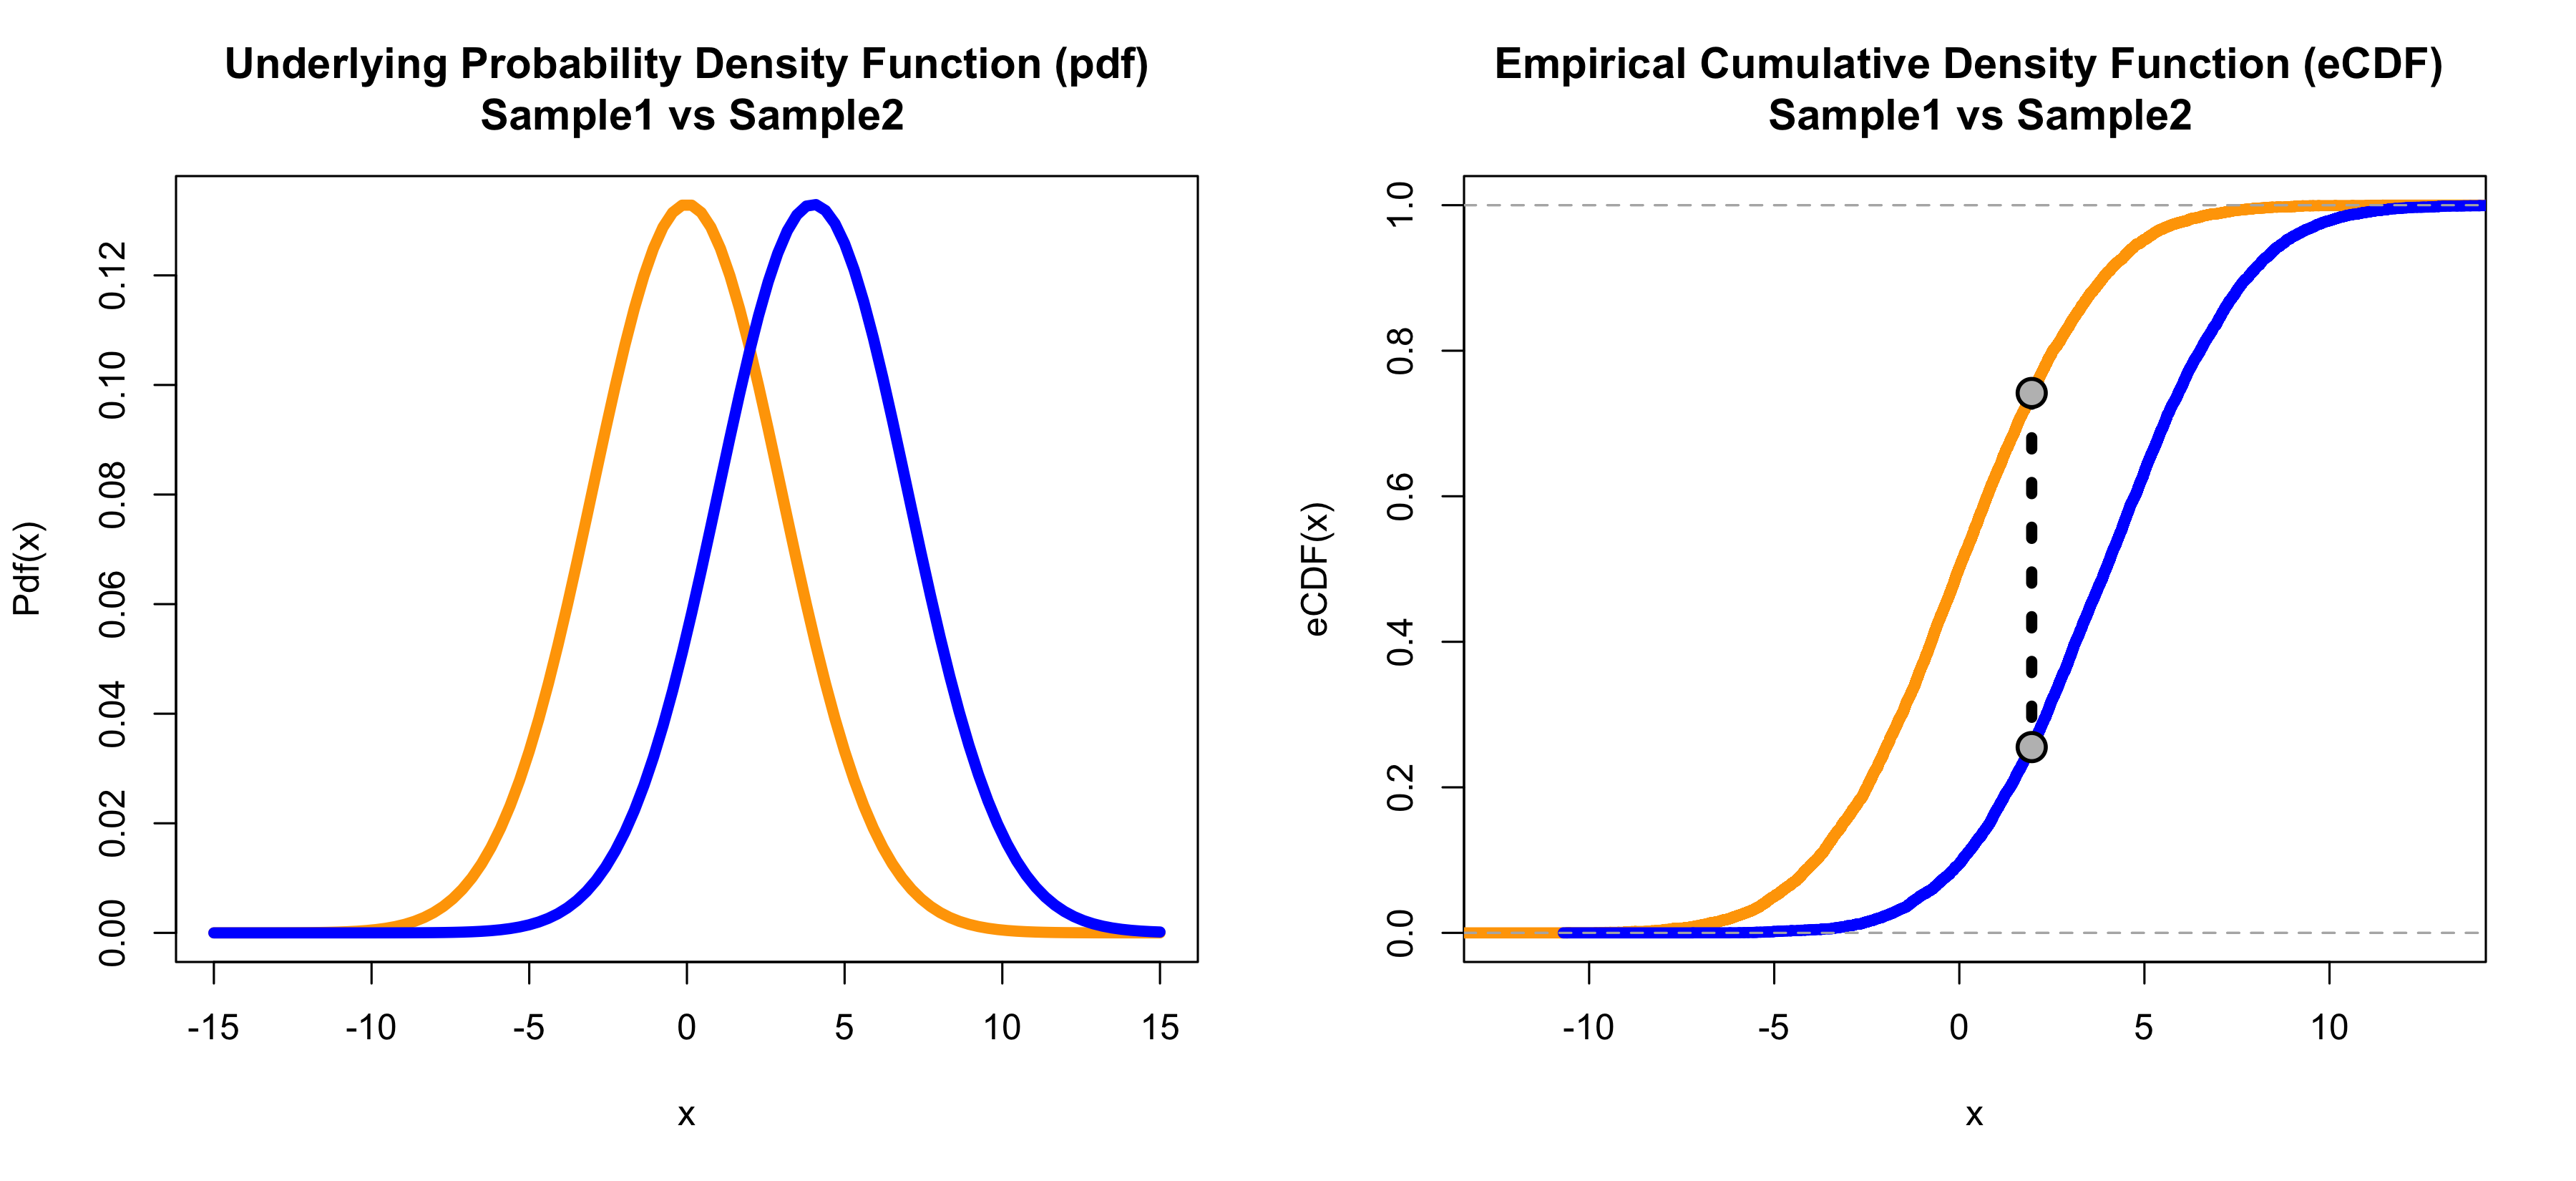
\includegraphics{pdfvsCDF}
\caption{\label{fig:kstest1D} \textbf{LEFT:} Probability density
function (PDF) of two normal distributions: orange sample~1,
$\mathcal{N}(\mu = 0,\,\sigma^{2} = 1)$; blue sample~2,
$\mathcal{N}(\mu = 5,\,\sigma^{2} = 1)$. \textbf{RIGHT:} Cumulative
density functions (CDF) of the two PDFs; the black dotted line
represents the maximal absolute difference between the CDFs
($D_{KS}$).  }
\end{figure}

In the large--sample limit ($n \geq 80$), it can be
shown~\citep{Kendall1946} that $D_{KS}$ converges in distribution to
\begin{equation} \label{eq:1}
D_{KS} \overset{d}{\rightarrow} \Phi(\lambda) = 2 \sum_{k=1}^{\infty} -1^{k-1}e^{-2k^2\lambda^2} \,.
\end{equation}
In the one-sample case with a sample of size $n$, the $p$~value is given by
\begin{equation} \label{eq:2}
\mathbb{P}(D > observed) = \Phi ( D\sqrt{n})\,;
\end{equation}
in the two-sample case, the $p$~value is given by
\begin{equation} \label{eq:3}
\mathbb{P}(D > observed) = \Phi \left( D\sqrt{\frac{n_1n_2}{n_1+n_2}} \right)\,.
\end{equation}
where $n_1$ and $n_2$ are the number of observations in the first and second samples respectively.

\subsection{Higher dimensional variations: Peacock Test (1983) and Fasano--Franceschini Test (1987)}
Extending the above to two or higher dimension is complicated by the
fact that CDFs are not well-defined in more than one dimension.  In
2-D, there are 4 ways (3 independent) of defining the cumulative
distribution, since the direction in which we order the $x$ and $y$
points is arbitrary (\textbf{Figure \ref{fig:kstest2Dissue}}); more
generally, in $k$-dimensional space there are $2^{k}-1$ independent
ways of defining the cumulative distribution
function~\citep{Peacock1983}.

\begin{figure}[t!]
\centering
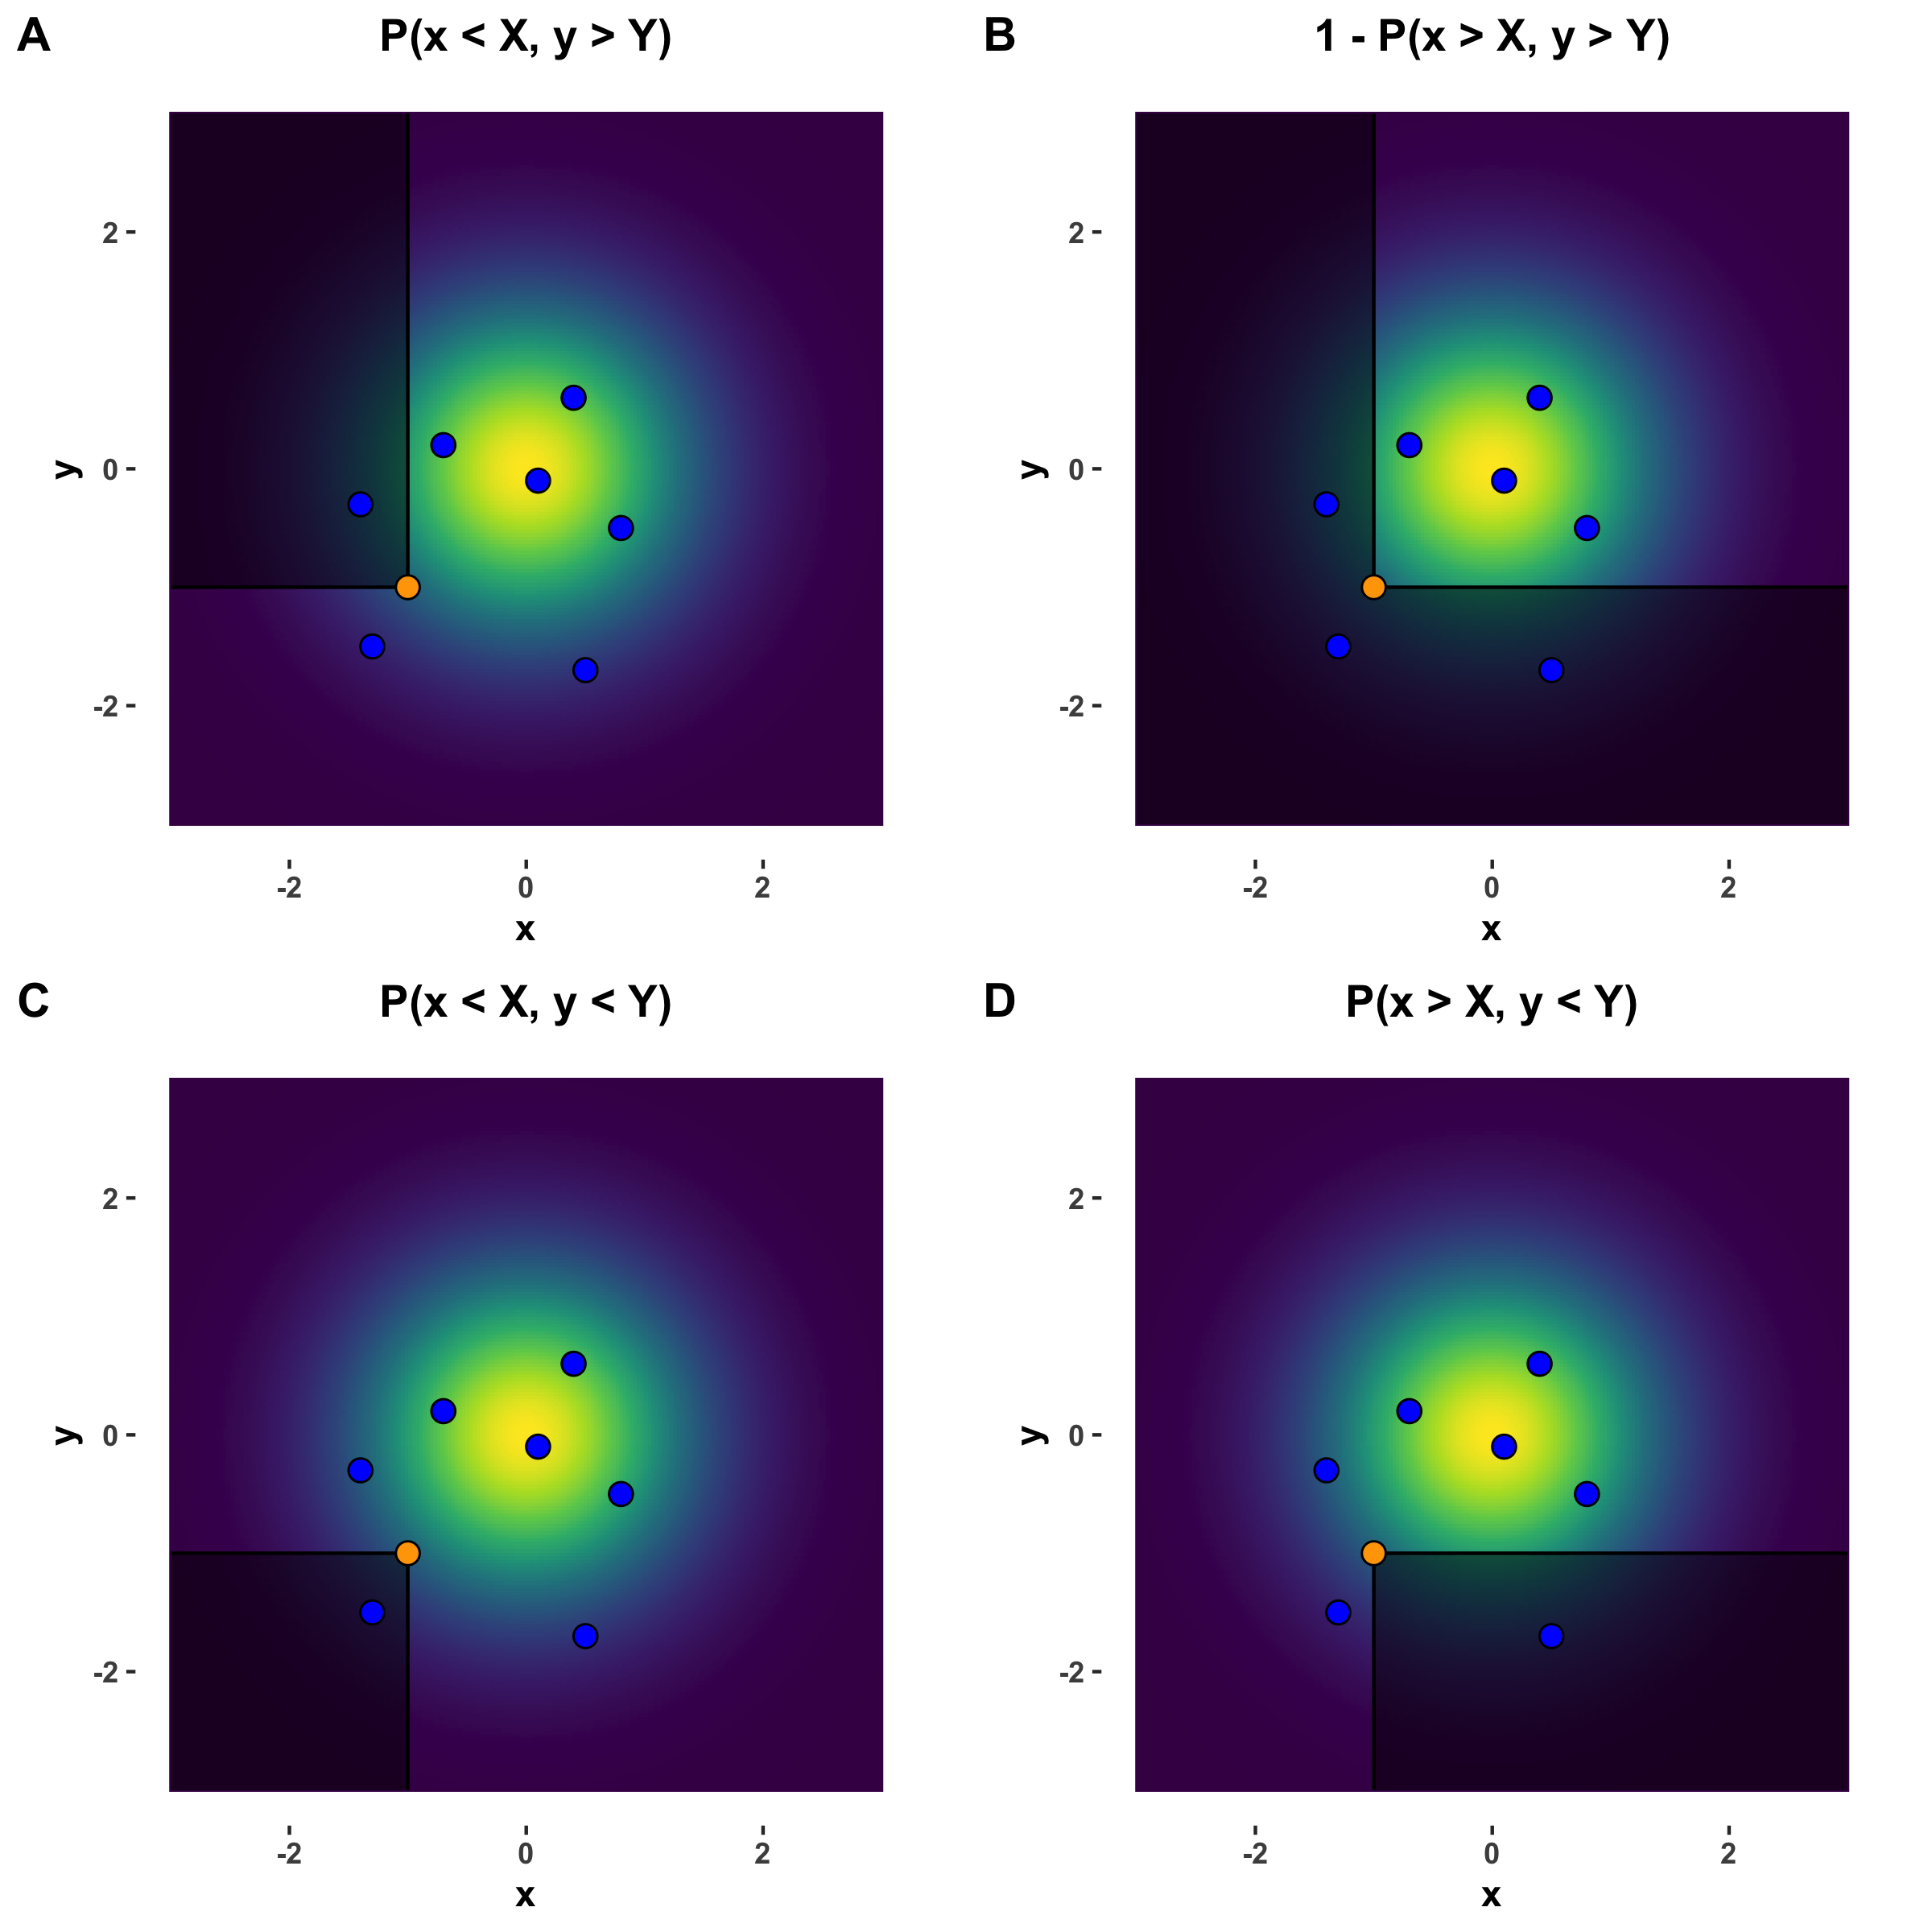
\includegraphics{CDF2Dissue}
\caption{\label{fig:kstest2Dissue} Four ways (3 independent) of defining the cumulative distribution for a given point in 2-D.  Here, the orange point $(X,Y)$ is chosen as the origin; the density of observations may be integrated as
$\mathbb{P}(x < X, y > Y)$ (A);
$\mathbb{P}(x < X \cup y < Y)$ (B);
$\mathbb{P}(x < X, y < Y)$ (C);
$\mathbb{P}(x > X, y > Y)$ (D).
}
\end{figure}

\cite{Peacock1983} solved the higher dimensionality issue by defining
the 2-D test statistic as the largest difference between the empirical
and theoretical cumulative distributions, after taking all possible
ordering combinations into account. Peacock's test thus computes the
total probability---i.e.\,fraction of data---in each of
the four quadrants around all possible tuples in the data. For
example, for $n$ points in a two-dimensional space, the empirical
cumulative distribution functions is calculated in the $4n^2$
quadrants of the plane defined by all pairs $(X_i, Y_j): i,j\in[1,n]$, where $X_i$ and
$Y_j$ are any observed value of $x$ and $y$ (whether or not they are observed as a pair).
There are $n^2$ such pairs, each of which can define four quadrants in the 2-D plane;
by ranging over all possible pairs of data points and quadrants, the
2-dimensional $D$ statistic is defined by the maximal difference of
the integrated probabilities between samples.

The variation defined by \cite{Fasano1987}  was to only consider
quadrants centered on each observed $(x, y)$ pair to compute the
cumulative distribution functions. That is, rather than looking over all $n^2$ points
${(X_i, Y_j): i,j \in [1,n]}$, Fasano and Franceschini only use the observed $n$ points
${(X_i, Y_i): i \in [1,n]}$.
Thus for any given $n$ points in a two-dimensional space, those $n$ points define $4n$ (rather than
$4n^2$) quadrants.  The proceedure is illustrated in \textbf{Figure~\ref{fig:kstest2D}}.
The algorithm loops through each point in one sample in turn to define
the origin of 4 quadrants (grey dotted lines in
\textbf{Figure~\ref{fig:kstest2D}}). The fraction of points in each
sample is computed in each quadrant, and the quadrant with the maximal
difference is designated with the current maximum for the specified
origin. By iterating over all data points and quadrants, the test
statistic $D_{FF,1}$ is defined by the maximal difference of the
integrated probabilities between samples in any quadrant for any
origin from the first sample.  In \textbf{Figure~\ref{fig:kstest2D}},
using the orange point as the origin, the maximal difference is
$D_{FF,1} = 0.52$.

\begin{figure}[t!]
\centering
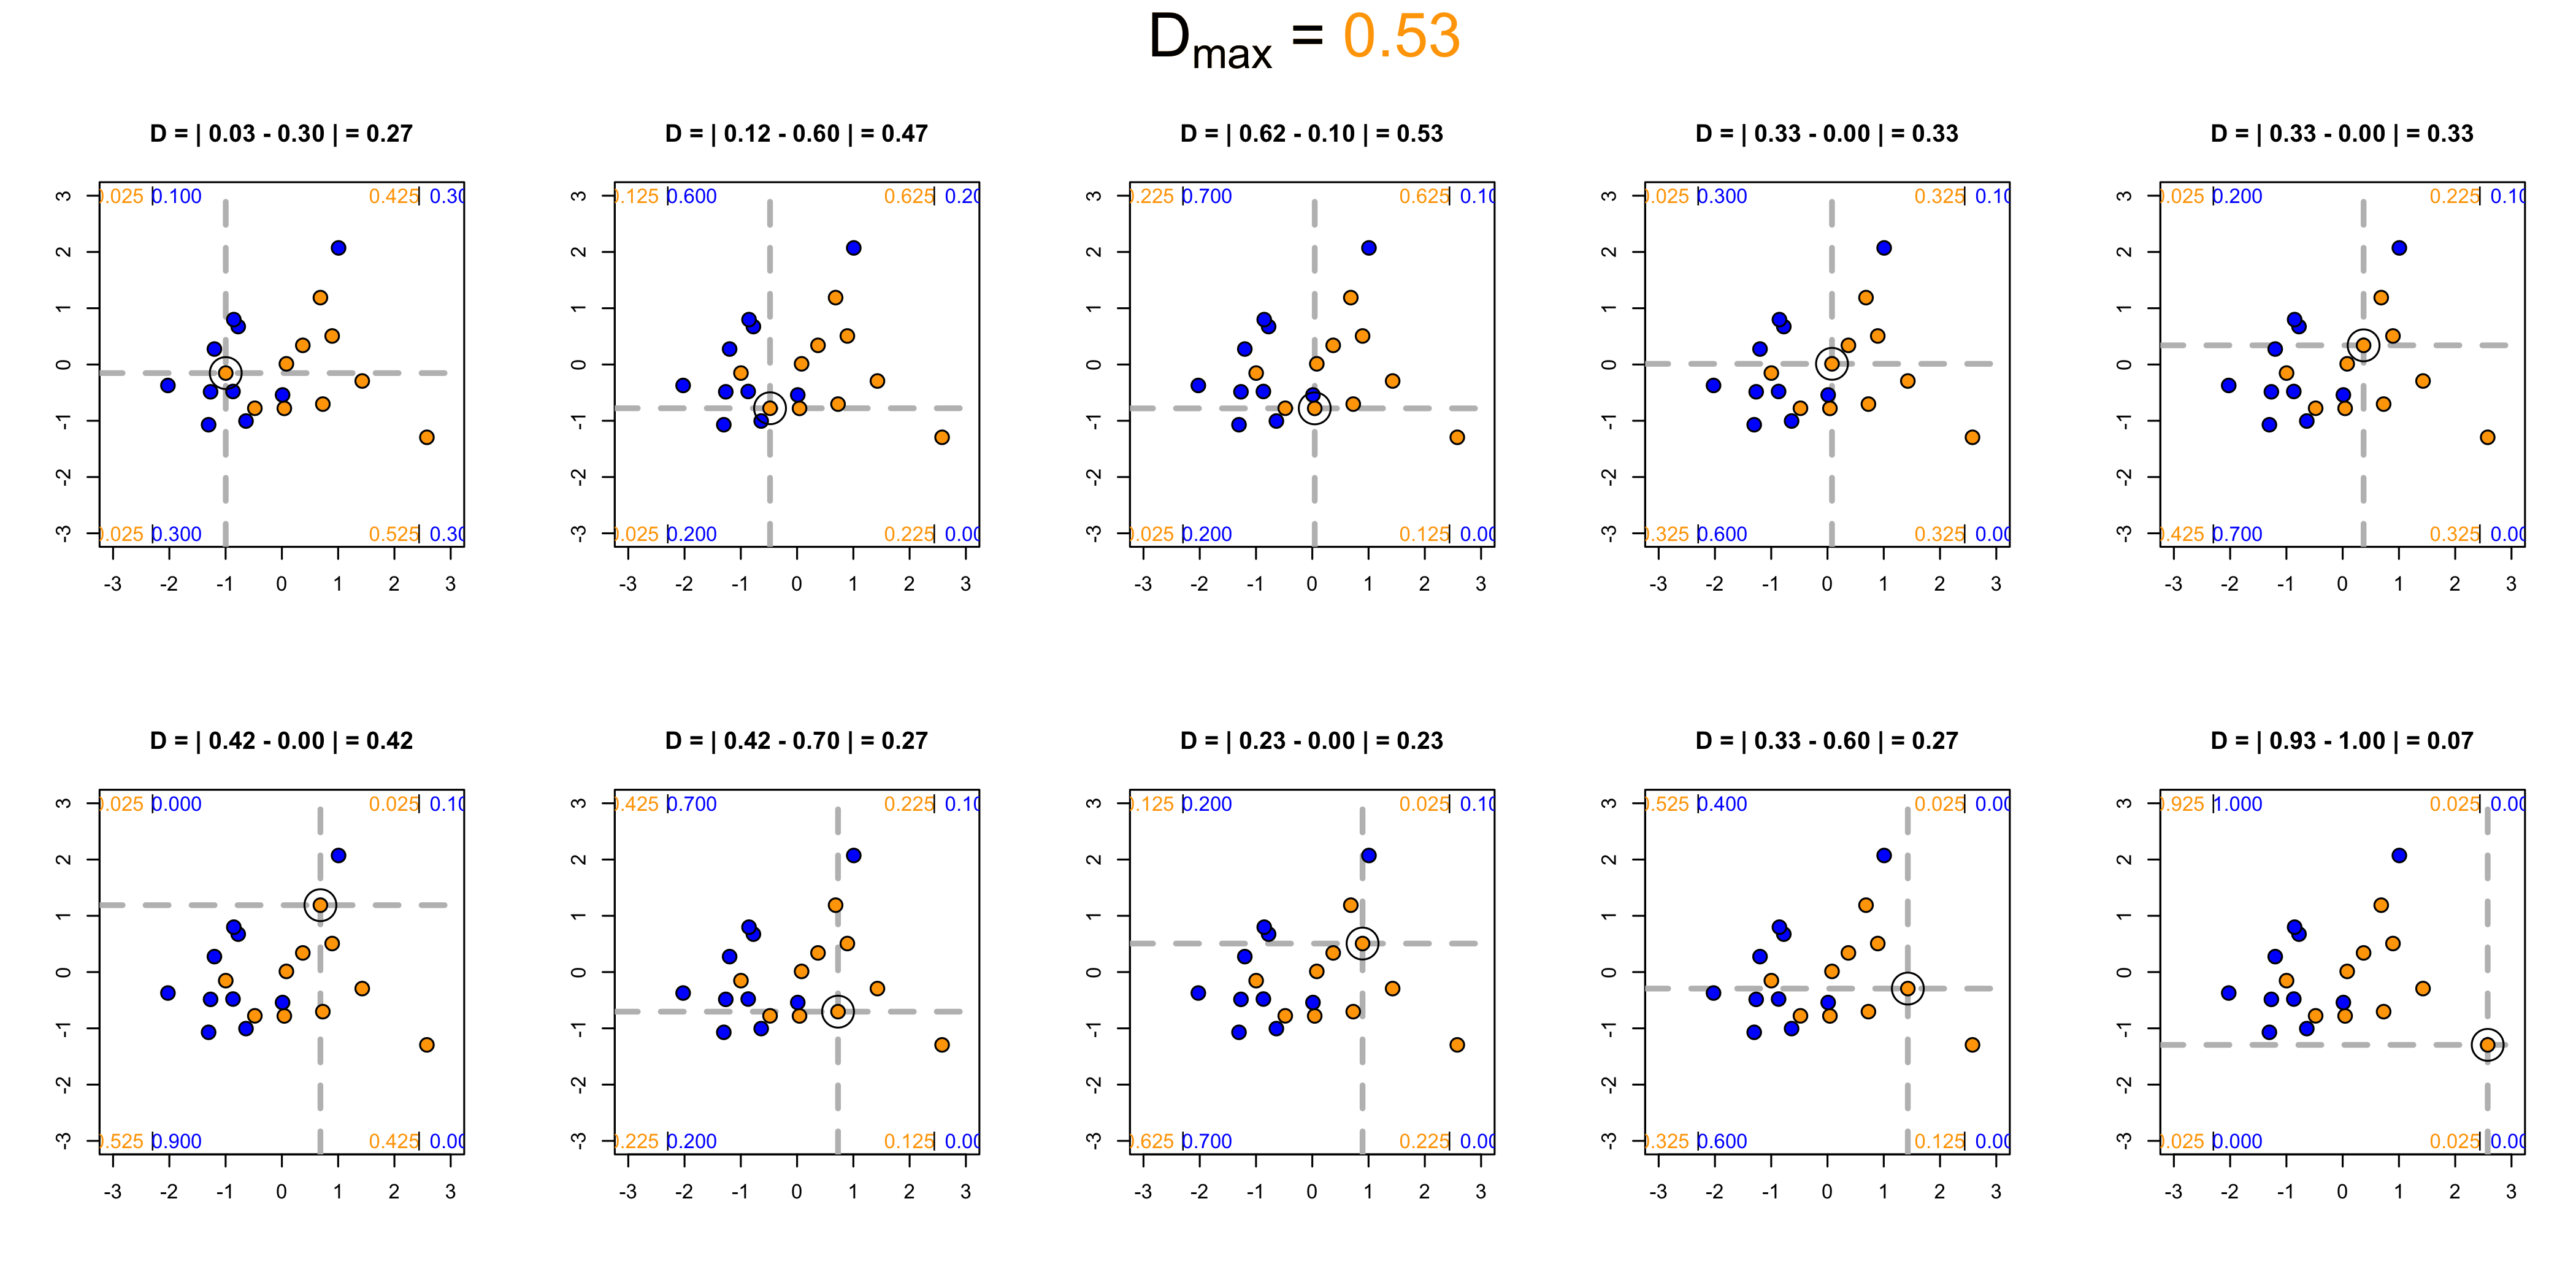
\includegraphics{fftestOutput}
\caption{\label{fig:kstest2D} Illustration of the Fasano--Franceschini algorithmic search for the maximal difference ($D_{FF,1}$) between sample 2-D eCDFs. Looping through each point in the sampled data to define a unique origin (grey dotted line), the fraction of orange and blue points in each quadrants are computed (plot corners). For each origin, the quadrant which maximizes the absolute difference in the integrated probabilities is indicated. The origin which maximizes the overall absolute difference in the integrated probabilities between samples is highlighted by the orange box.
}
\end{figure}

%\RBnote{Since $D_{FF}$ from one sample isn't the final $D_{FF}$, you should note it appropriately (eg, $D_{FF,1}$ and $D_{FF,2}$). - ENC: Text has been updated accordingly}
This process is repeated using the points from \textit{other} sample
as the origins to compute the maximal $D_{FF,2}$ with origins from the
second sample. $D_{FF,1}$ and $D_{FF,2}$  are then averaged to compute
the overall $D_{FF}$ for hypothesis testing,
$D_{FF}=(D_{FF,1}+D_{FF,2})/2$.

It may be that some points are tied with the $X$ and/or $Y$
coordinates of the origin, creating an ambiguity when computing the
fraction of points in each quadrant. Since the
test attempts to define the maximal difference of the cumulative
probabilities, a natural solution would be to treat a point that is
tied with the current $X$ and/or $Y$ coordinates of the origin as equally
likely to have been drawn from any of the tied quadrants.
Hence, any data point
sharing the same $X$ or $Y$ coordinate as the origin is evenly
distributed across the tied quadrants, with each of the two quadrants
receiving half a count. Any data point sharing the both the same $X$ and $Y$
coordinates as the current origin (including the origin itself) is evenly
distributed across all quadrants, with all four quadrants receiving a
quarter count.

\subsection{Null distribution of $D_{FF}$}

Using Monte Carlo simulation, Fasano and Franceschini created a
look-up table of critical values of $D_{FF}$ as a function of
$D_{FF}$, the sample size, and the coefficient of correlation $r$.
\cite{numericalRecipes} later defined an approximate fit to the lookup table
as follows.
%
For a single sample of size $n$,
\begin{equation} \label{eq:4}
\mathbb{P}(d_{FF} > D_{FF}) = \Phi \left( \frac{D_{FF}\sqrt{n}}{1+\sqrt{1-r^2}(0.25-0.75/\sqrt{n})} \right) \, .
\end{equation}
where $\Phi(\cdot)$ is as defined in Eq~\ref{eq:1}.
The two sample case uses the same formula as above, but with the slight variation where
\begin{equation} \label{eq:5}
n = \frac{n_1n_2}{n_1+n_2}\, .
\end{equation}
In both cases, $r$ is defined in the usual way as
\begin{equation} \label{eq:6}
r = \frac{\sum_{i}(X_i-\bar{X})(Y_i-\bar{Y})}{\sqrt{\sum_{i}(X_i-\bar{X})^2}\sqrt{\sum_{i}(Y_i-\bar{Y})^2}}\, .
\end{equation}


\section{Illustrations} \label{sec:illustrations}

\subsection{Fasano--Franceschini test usage}

In their paper, Fasano and Franceschini use Monte Carlo simulation to
approximate the distribution of $D_{FF}$ as a function of the sample
size $n$ and the coefficient of correlation $r$. Notably, unlike the 1-D KS
test, the distribution of
$D_{FF}$ is \textit{not} completely independent of the shape of the 2-D distribution of the
underlying data, but depends on the correlations between the variables.
In the case where the variables $X$ and $Y$  are perfectly
correlated ($r = 1$), the 2-D distribution lies along a single line and thus
the 1-D KS test could be used; at the other extreme were $X$ and $Y$  are perfectly
uncorrelated ($r = 0$), the 2-D distribution is independent in the $X$
and $Y$ directions and one could apply the 1-D KS test on the marginal
distributions.
%
Results from Monte Carlo simulation support these expectations, showing
that the distribution of $D$ is nearly identical for varying
distributions with the same correlation coefficient~\citep{Fasano1987}.
The approximation
by  \cite{numericalRecipes} (Eq~\ref{eq:4}--\ref{eq:5})
can be used to test the significance levels for the 2-D K-S test using
the following code:
%
\begin{CodeChunk}
\begin{CodeInput}
R> #set seed for reproducible example
R> set.seed(123)
R>
R> #create 2-D samples with the same underlying distributions
R> sample1Data <- data.frame(
R>  x = rnorm(n = 100, mean = 0, sd = 1),
R>  y = rnorm(n = 100, mean = 0, sd = 1)
R> )
R> sample2Data <- data.frame(
R>  x = rnorm(n = 100, mean = 0, sd = 1),
R>  y = rnorm(n = 100, mean = 0, sd = 1)
R> )
R>
R> fasano.franceschini.test(sample1Data,sample2Data)
\end{CodeInput}
\begin{CodeOutput}
      2-D Two-sample Kolmogorov-Smirnov Test

 Fasano--Franceschini Test (1987)
 Data:  sample1Data and sample2Data
 D-stat =  0.14 , p-value =  0.4420642
 Run Time (s) =  0.06367922
\end{CodeOutput}
\end{CodeChunk}

\subsection{Bootstrap version of the Fasano--Franceschini test}

It has been noted that the approximation from
\citet{numericalRecipes} is only accurate when $n \gtrsim 20$ and the
$p$-value is less than (more significant than) $\sim 0.2$
\citep{Babu2006}. While this inaccuracy still allows a simple
rejection decision to be made at any $\alpha\leq0.2$, it is sometimes
useful to quantify large $p$ more exactly (such as if one was to do a
cross-study concordance analysis comparing $p$~values between studies
as in~\cite{Ness-Cohn2020}), and to apply it to smaller datasets.
%
To address these limitations, one can bootstrap the significance
levels for the particular multidimensional statistic directly from the
particular data set under study. As Fasano and Franceschini's paper
was originally released in 1987, this approach was unfeasible at
scale.  Today, modern computers can rapidly compute a bootstrapped
null distribution of $D_{FF}$ from the data to test significance.

The \pkg{fasano.franceschini.test} R package implements a parallelized
bootstrapping procedure. The marginal distribution from 2-dimensional
data set is resampled with replacement to generate randomized
2-dimensional data sets \code{nBootStrap} times. The frequency count
by quadrant is performed for each bootstrapped resampling as described
above to compute the $D_{FF}$. The observed $D_{FF}$ is then compared
to the distribution of bootstrapped $D_{FF}$ to compute a $p$~value.
The bootstrapped version of the Fasano--Franceschini test can be
run as follows (see \fct{fasano.franceschini.test} for further
source code details and implementation).

\begin{CodeChunk}
\begin{CodeInput}
R> #set seed for reproducible example
R> set.seed(123)
R>
R> #create 2-D samples with the same underlying distributions
R> sample1Data <- data.frame(
R>  x = rnorm(n = 100, mean = 0, sd = 1),
R>  y = rnorm(n = 100, mean = 0, sd = 1)
R> )
R> sample2Data <- data.frame(
R>  x = rnorm(n = 100, mean = 0, sd = 1),
R>  y = rnorm(n = 100, mean = 0, sd = 1)
R> )
R>
R> fasano.franceschini.test(S1 = sample1Data, S2 = sample2Data,
R>                          nBootstrap = 1000, cores = 1)
\end{CodeInput}
\begin{CodeOutput}
      2-D Two-sample Kolmogorov-Smirnov Test

 Fasano--Franceschini Test (1987)
 Data:  sample1Data and sample2Data
 D-stat =  0.14 , p-value =  0.62
 Run Time (s) =  12.59964
\end{CodeOutput}
\end{CodeChunk}
To improve run time, one may adjust the \code{cores} parameter; see the R \pkg{parallel} package and the \fct{mclapply} function for further details.

\subsection{Computational efficency}

\begin{figure}[hbt]
\centering
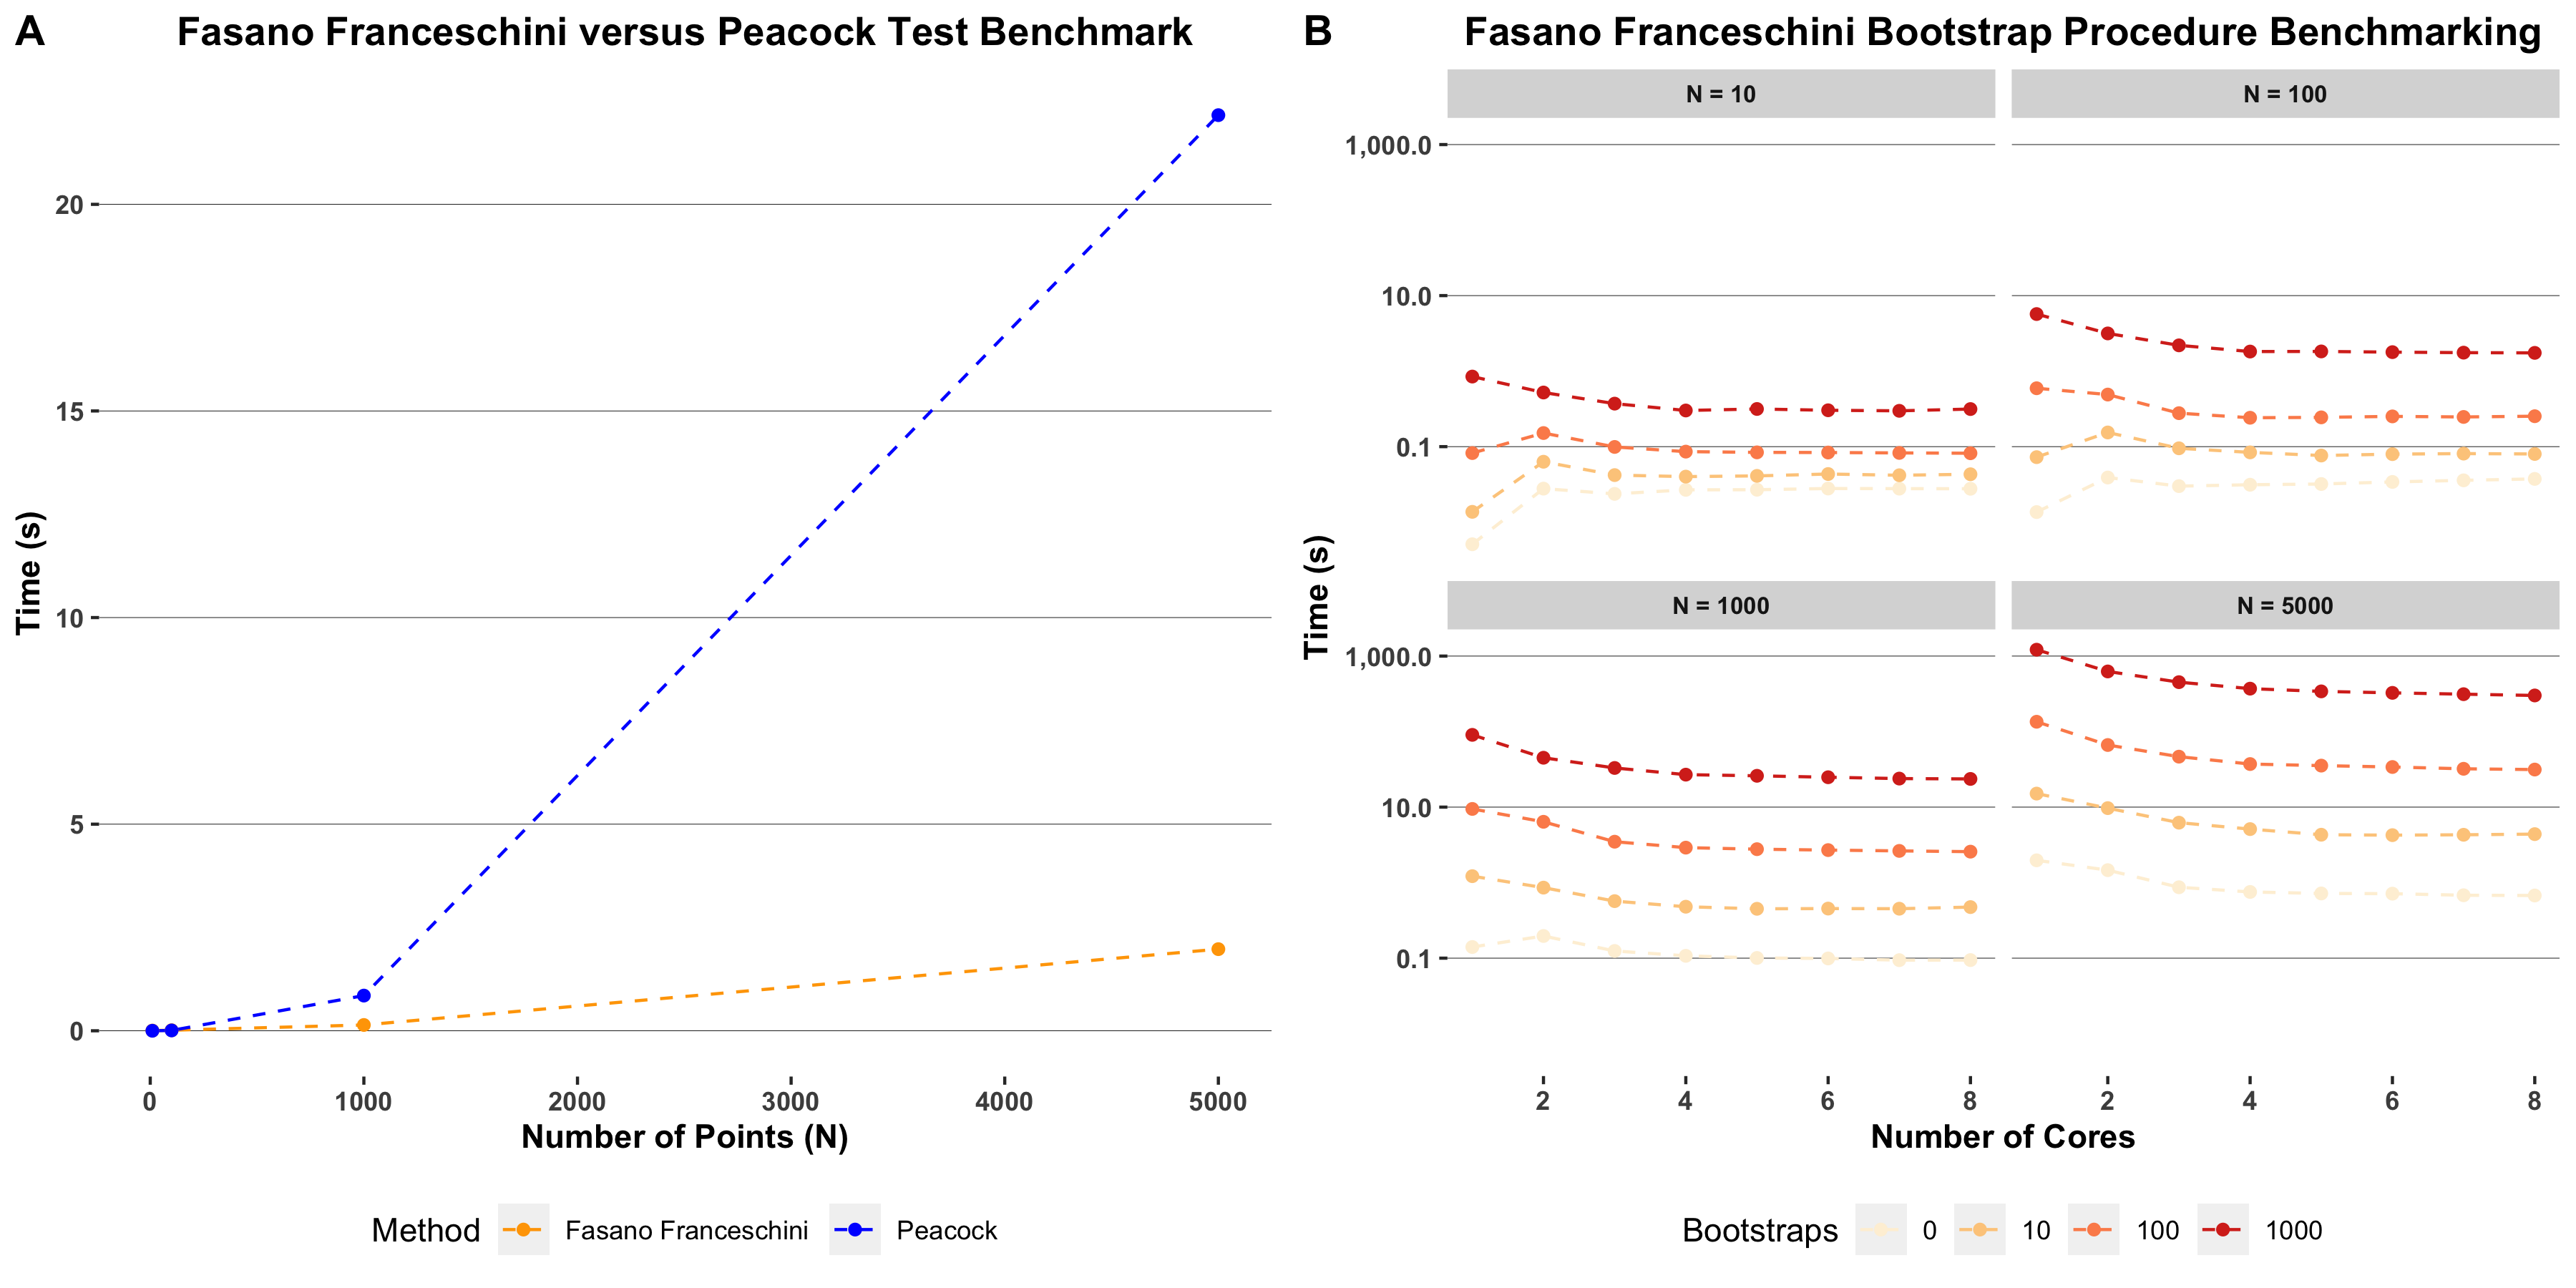
\includegraphics{benchmark}
\caption{\label{fig:bmark} Computational efficiency benchmarks.
\textbf{A:} Runtime of the
Fasano--Franceschini test relative to the Peacock test at four different sample sizes
($n=10, 100, 1000, 5000$).  Points represent the
average of 10 benchmark runs. \textbf{B:} Runtime of the
Fasano--Franceschini bootstrapping procedure for various sample sizes
($n= 10, 100, 1000, 5000$) as a function of the number of cores used. Within each panel,
lines are colored by the number of bootstrap iterations (no bootstrap, 10, 100,
1000). Points represent the average of 10 benchmark runs. Note the logarithmic $y$-axis
in (B).}
\end{figure}

To assess the computational efficiency, we benchmarked the package as follows.
Using the \pkg{rbenchmark} package to evaluate runtime, the Fasano--Franceschini
test and Peacock test were run under four different samples sizes
($n=10, 100, 1000, 5000$), with 10 replicates for each run. The
Fasano--Franceschini test bootstrap precedure was further evaluated
under four different bootstrap iterations (no bootstrap, 10, 100, 1000),
again using 10 replicates for each run. Reported results represent the
average run time of the 10 replicate benchmarks. All benchmark tests were run on a 2018 macBook
Pro Mac (macOS Catalina) with a 2.7-GHz Quad-Core Intel Core i7 processor and 16 GB of 2133 MHz LPDDR3 memory.

The main distinction between the Peacock and Fasano--Franceschini
tests is in computational efficiency, with  Fasano--Franceschini
scaling as $O(n^2)$ relative to Peacock's complexity of  $O(n^3)$
\citep{Lopes2007}.  Our benchmarks also show this advantage, as shown
in \textbf{Figure~\ref{fig:bmark}A}.  While the implentation of the
bootstrapping procedure increases runtime in comparison to the
approximate fit from  \citet{numericalRecipes}, parallelization of the
Fasano--Franceschini test shows a four-fold reduction in run time when
parallelized across 8 cores (\textbf{Figure~\ref{fig:bmark}B}).
% (See the \pkg{Peacock.test} package for \proglang{R} implementation of the Peacock test.)


%% -- Summary/conclusions/discussion -------------------------------------------

\section{Summary and discussion} \label{sec:summary}

The \pkg{fasano.franceschini.test} package is an \proglang{R} implementation of the 2-D two-sample KS test as defined by Fasano and Franceschini~\citep{Fasano1987}.
It improves upon existing packages by implementing
  a fast algorithm and
  a parallelized bootstrapping procedure for improved statistical testing.
  Complete package documentation and source code is available via the Comprehensive
\proglang{R} Archive Network (CRAN) at
\url{https://CRAN.R-project.org/} and the package website at \url{https://nesscoder.github.io/fasano.franceschini.test/}.


%% -- Optional special unnumbered sections -------------------------------------

\section*{Computational details}

% \begin{leftbar}
% If necessary or useful, information about certain computational details
% such as version numbers, operating systems, or compilers could be included
% in an unnumbered section. Also, auxiliary packages (say, for visualizations,
% maps, tables, \dots) that are not cited in the main text can be credited here.
% \end{leftbar}

The results in this paper were obtained using
\proglang{R}~4.0.3 with the
\pkg{fasano.franceschini.test}~1.0.0 package. \proglang{R} itself
and all package dependencies (\pkg{methods}~4.0.3; \pkg{parallel}~4.0.3) are available from the Comprehensive
\proglang{R} Archive Network (CRAN) at
\url{https://CRAN.R-project.org/}.

%\RBnote{Any other package dependencies? - ENC: added dependenceis parallel and methods}

\section*{Acknowledgments}

Research reported in this publication was supported by the NSF-Simons Center for Quantitative Biology at Northwestern University, an NSF-Simons MathBioSys Research Center. This work was supported by a grant from the Simons Foundation/SFARI (597491-RWC) and the National Science Foundation (1764421). The content is solely the responsibility of the authors and does not necessarily represent the official views of the National Science Foundation and Simons Foundation.

E.N.C developed the \pkg{fasano.franceschini.test} package and produced the tutorials/documentation; E.N.C.\,and R.B.\,wrote the paper.


%% -- Bibliography -------------------------------------------------------------
%% - References need to be provided in a .bib BibTeX database.
%% - All references should be made with \cite, \citet, \citep, \citealp etc.
%%   (and never hard-coded). See the FAQ for details.
%% - JSS-specific markup (\proglang, \pkg, \code) should be used in the .bib.
%% - Titles in the .bib should be in title case.
%% - DOIs should be included where available.

\bibliography{refs}
\newpage

\end{document}
